%%%%%%%%%%%%
% Mẫu để các bạn làm slides trình chiếu khi thuyết trình.
% Tôi chỉ lấy phần đơn giản nhất của gói lệnh beamer hướng dẫn
% Các bạn tự tìm hiểu sau này.
% Tác giả tài liệu này: Nguyễn Hữu Điển
%  Khoa Toán - Cơ - Tin học
 % Đại học Khoa học Tự nhiên Hà nội
%Email: huudien@vnu.edu.vn, 
%%%%%%%%%%%%%
\documentclass[10pt,notheorems]{beamer}
\usepackage{amsmath,amsxtra,amssymb,latexsym, amscd,amsthm}
\usepackage{indentfirst}
\usepackage[mathscr]{eucal}
\usepackage{graphicx}
\usepackage{color}
\usepackage[utf8]{vietnam}
\usepackage{graphics}
\usepackage{ucs}
\usepackage{picinpar}
\usepackage{floatflt}
\usepackage{commath}
\usepackage{makeidx}
\usepackage{enumerate}
\usepackage{longtable}%
\usepackage{multicol}%
%\usetheme{split}
%\usepackage{beamerthemesplit}
%\usepackage{beamerthemesidebar}
%\usetheme{Warsaw}
% \usetheme{bergen}
\usetheme{Madrid}
 %\usetheme{boadilla}
%\setbeamercovered{transparent}
\newcommand{\R}{\mathbb{R}}
%\newcommand{\C}{\mathbb{C}}
\newcommand{\N}{\mathbb{N}}
\newcommand{\K}{\mathbb{K}}

\usepackage[english]{babel}
\usepackage{listings}
\newtheorem{dly}{Định lý}
\newtheorem{mde}[dly]{Mệnh đề}
\newtheorem{bde}[dly]{Bổ đề}
\newtheorem{hqua}[dly]{Hệ quả}

\theoremstyle{definition}
\newtheorem{dng}{Định nghĩa}
\newtheorem{nx}{Nhận xét}
\newtheorem{gch}[dly]{Chú ý}
\newtheorem*{cm}{Chứng minh}

\theoremstyle{definition}
\newtheorem{vd}[dly]{Ví dụ}
\newtheorem{bt}[dly]{Bài toán}
\newtheorem{pp}[subsection]{Phương pháp}

\theoremstyle{definition}
\newtheorem{tch}[dly]{Tính chất}

\def\n{\noindent}
\def\N{\mathbb{N}}
\def\R{\mathbb{R}}
\def\p{\varphi}
\def\cc{\mathcal }
\def\ov{\overline}
\def\a{\alpha}
\def\lb{\lambda}
\def\va{\varepsilon}
\def\g{\gamma}
\DeclareMathOperator{\intt}{int}
\newcommand{\m}[1]{
	\begin{bmatrix}
		#1
\end{bmatrix}}
\def\cA{\mathcal{A}}
\def\cC{\mathcal{C}}
\def\cP{\mathcal{P}}
\def\tu{\tilde{u}}
\def\R{\mathbb{R}}
\def\C{\mathbb{C}}
\newcommand{\pma}[1]{
	\begin{matrix}
		#1
\end{matrix}}
%%%%%%%%%%%%%%%%%%%%%%%%%1
\author{HỌC VIÊN: HOÀNG VIỆT ANH}
\institute[Khóa: 2015-2018]{\bf {}\\
	Khoa Toán - Tin\\
	Trường Đại học Sư phạm Hà Nội\\
	\vspace{0.5cm}
	TIỂU LUẬN TỔNG QUAN}
\title{LÝ THUYẾT ĐIỀU KHIỂN \\ CỦA CÁC HỆ ĐỘNG LỰC CÓ TRỄ \\ SỬ DỤNG PHƯƠNG PHÁP HÀM LAMBERT \\ VÀ ỨNG DỤNG}
%\title{TÍNH ỔN ĐỊNH VỮNG CỦA MỘT SỐ LỚP HỆ CHUYỂN MẠCH TUYẾN TÍNH}
\institute[]{\bf HƯỚNG DẪN: TS. HÀ PHI \quad \quad  \quad \quad\\
	\vspace{1cm}
	\large{Khoa: Toán - Tin, Trường Đại học Sư phạm Hà Nội}
	}
\date{Hanoi, 10/07/2020}
\begin{document}
	
\AtBeginSection[]{
\begin{frame}
\tableofcontents[currentsection]
\end{frame}
}

	
\frame{\maketitle}
\mode<presentation>{\setbeamertemplate{theorems}[numbered]}
%\subject{Presentation Programs}


\begin{frame}{Lý do chọn đề tài}
	\begin{itemize}
		\item Hệ điều khiển có trễ 
		\begin{align*}
			\dot{x}(t)&=ax(t)+a_dx(t-h)+bu(t)\\
			y(t)&=  C x(t)
		\end{align*}
		nảy sinh từ rất nhiều ứng dụng trong thực tế và vẫn đang được quan tâm nghiên cứu,
		\item Cách tiếp cận sử dụng hàm Lambert $$W(z)e^{W(z)}=z$$
		mới lại được quan tâm nhiều trong vòng 10 năm trở lại đây,
		\item Toolbox lambertWDDE (version 1.0, 2012): phân tích các tính chất 
		ổn định và điều khiển của hệ điều khiển có trễ thông qua hàm Lambert W,
		được viết trong MATLAB.
				
	\end{itemize}
\end{frame}


\begin{frame}{\centerline {Nội dung}}
\tableofcontents
\end{frame}
%%%%%%%%%%%%%%%%%%%%%%%%%%%%%%%%%%%%%%%%%%%
\section{Một số kiến thức cơ sở}
%%%%%%%%%%%%%%%%%%%%%%%%%%%%%%%%%%%%%%%%%

\subsection{Sơ lược về hàm Lambert W}

\begin{frame}{Sơ lược về hàm Lambert W}
\begin{block}{Hàm Lambert W}
Mọi hàm $W(s)$ thỏa mãn:
\begin{equation}\label{2}
W(s)e^{W(s)}=s
\end{equation}
được gọi là hàm Lambert W. Hàm Lambert W, với đối số phức $s$, là một hàm có giá trị phức với các nhánh vô hạn, $k=0,\pm 1,\pm 2,...,\pm\infty$ ở đây
$s$ là một số (tức là hàm vô hướng Lambert W) hoặc ma trận (tức là, hàm ma trận Lambert W).
\end{block}
\end{frame}


\begin{frame}{}
\begin{minipage}{6.5cm}
\begin{block}{Tính chất của hàm Lambert vô hướng}
1. Hàm Lambert $W$ là hàm có giá trị phức đối với đối số phức $z$ và nó có vô hạn nhánh $W_{k}$, ở đó $k = 0,\pm 1,\pm 2,...,\pm\infty$\\\pause
2. Hàm Lambert $W$ có hai nhánh thực với điểm nhánh là $(-e^{-1},-1)$\\\pause
3. Ngoại trừ điểm $z=-e^{-1}$ mà nhánh chính $W_0$ không khả vi, tất cả các nhánh đều là giải tích địa phương\\\pause
4. 	$ W'(x) = \dfrac{1}{x+e^{W(x)}} = \dfrac{W(x)}{x \ (1+W(x))} \ .$ \pause
5. Python, Matlab, Maple, Mathematica, ... đều có hàm Lambert (vô hướng).\pause
\end{block}	
\end{minipage}
\hfill
\begin{minipage}{5cm}
			\begin{figure}[h]
			\centering
			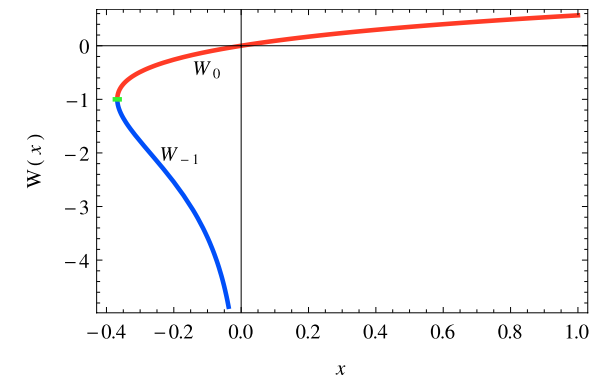
\includegraphics[scale=0.3]{hinh/Screenshot_1}
			\caption{Hàm Lambert với 2 nhánh chính k=0, k=-1}
			\label{fig1}
		\end{figure}
	\end{minipage}
\end{frame}


\begin{frame}{}
\begin{block}{Dạng ma trận của hàm Lambert}
Dựa trên dạng chuẩn tắc Jordan
$$ J=\text{diag}(J_{n_1}(\lambda_1),J_{n_2}(\lambda_2),\cdots,J_{n_s}(\lambda_s))$$
với $J_n(\lambda)$ là ma trận Jordan cỡ $n\times n$ tương ứng với giá trị riêng $\lambda$ bội $n$.\pause \\

Đặt \hspace{0.9cm} $W_k(J)=\text{diag}(W_{k_1}(J_{n_1}(\lambda_1)),W_{k_2}(J_{n_2}(\lambda_2)),\cdots,W_{k_s}(J_{n_s}(\lambda_s))).$
$$ W_k(J_n(\lambda))=\begin{bmatrix}
W_k(\lambda)&W_k^\prime(\lambda)&\cdots & \dfrac{1}{(n-1)!}W_k^{(n-1)}(\lambda)\\
& W_k(\lambda) & \ddots & \vdots\\
& & \ddots & W_k^\prime(\lambda)\\
& &  & W_k(\lambda)
\end{bmatrix}
\ .
$$\pause
\end{block}
\begin{block}{Tổng quát}
	$$W_k(A)=SW_k(J)S^{-1}.$$
\end{block}
\end{frame}


\begin{frame}{}
	\begin{block}{Chú ý}
\begin{itemize}
\item Nếu $k=0$ thì ta phải giả sử thêm là $\lambda\neq -e^{-1}$ (vì $W_0^\prime(-e^{-1})$ không xác định) 
\item Với nhánh chính $k=0$, từ bây giờ ta sẽ giả sử rằng $-e^{-1}$ không phải là giá trị riêng tương ứng với khối Jordan với số chiều lớn hơn 1, tức là
$$\text{rank}(A+e^{-1}I)=\text{rank}(A+e^{-1}I)^2.$$
\end{itemize}
\end{block}
\end{frame}


\begin{frame}{}
\begin{block}{Ví dụ 1.1}\label{vd1.1}
	Xét ma trận
	%
	\[
	A = \m{1 & 1 & 1 \\ 0 & 1 & 2 \\ 0 &  0  &  3}. 
	\]
	%
	Phân tích Jordan của ma trận A là $A = S J S^{-1}$, trong đó
	%
	\[
	S = \m{ 1 &  -2 & -1 \\ 1 &    0  &  -2 \\ 	1  &   0  &   0 }, \quad J = \m{3 &  0 & 0 \\ 0 &  1 &  1 \\ 0 &  0 & 1} \ .
	\]
	%
	Nếu ta chọn $k_1  = 0$, $k_2 = 2$ tương ứng với hai block Jordan, khi đó ta có 
	%
	\[
	W_k(A) = S \m{W_0(3) & 0  \\ 0  & W_2\left( \m{1 &  1 \\ 0 &  1} \right) } S^{-1} 
	= S \m{W_0(3) & 0 & 0 \\ 0  & W_2(1) & W'_2(1) \\  0 & 0  & W_2(1)} S^{-1} \ .
	\]
\end{block}
\end{frame}

\subsection{Một số tính chất cơ bản của các hệ điều khiển không trễ}

\begin{frame}{Một số tính chất cơ bản của các hệ điều khiển không trễ}
Xét một hệ điều khiển không trễ dạng
%
\begin{equation}\label{1}
\begin{split}
\dot{x}(t) &= Ax(t)+Bu(t), \\
y(t) &= Cx(t) + Du(t),
\end{split}
\end{equation}
\begin{block}{Định nghĩa 1}
	i) Hệ \eqref{1} hay cặp $(A,B)$ được gọi là \emph{điều khiển được} nếu với mọi trạng thái ban đầu $x(0)=x_0$ và trạng thái cuối $x_1$, tồn tại một hàm điều khiển để truyền từ trạng thái $x_0$ sang trạng thái $x_1$ trong thời gian hữu hạn $t_1>0$, tức là $x(t_1) = x_1$. \\
	ii) Hệ điều khiển \eqref{1} hay cặp $(A,C)$ được gọi là \emph{quan sát được} nếu với mọi trạng thái ban đầu $x(0)=x_0$ chưa biết, tồn tại một thời điểm $t_1 > 0$ sao cho $x_0$ có thể được xác định duy nhất dựa trên hàm điều khiển $u(t)$ và hàm đầu ra $y(t)$ trên đoạn $[0,t_1]$. 
\end{block}	
\end{frame}




\begin{frame}{}
\begin{block}{Định nghĩa 2} Xét hệ điều khiển \eqref{1}. Khi đó  ma trận 
	%
	\[
	W_c(t) : = \int_{0}^{t} e^{A(t-s)} B B^T e^{A^T (t-s)}ds
	\]
	%	
được gọi là \emph{ma trận điều khiển Gramian}.
\end{block}

\begin{block}{Định lý 1.2 (Chen.98)}
	Hệ \eqref{1} là điều khiển được khi và chỉ khi một trong những điều kiện tương đương sau được thỏa mãn.
	\begin{enumerate}
		\item[i)] Ma trận điều khiển Gramian $W_c(t)$ là khả nghịch với mọi $t>0$. 
		\item[ii)] Ma trận điều khiển được
		%
		\[
		\cC := \m{B & AB & A^2B & \dots & A^{n-1} B}
		\]
		%
		là đủ hạng dòng.
		\item[iii)] Ma trận $\m{A-\lb I_n & B}$ là đủ hạng dòng với mọi $\lb \in \mathbb{C}$.
	\end{enumerate}
\end{block}	
\end{frame}

%%%%%%%%%%%%%%%%%%%%%%%%%%%%%%%%%%%%%%%
\section{Ứng dụng hàm Lambert W trong lý thuyết phương trình vi phân có trễ}
\subsection{Trường hợp vô hướng}

\begin{frame}{Phương trình vô hướng}
Xét hệ điều khiển 
%
\begin{equation}\label{3}
\dot{x}(t)=ax(t)+a_dx(t-h)+bu(t),
\end{equation} \pause
%
trong đó $a$, $b$, $a_d$ là các hằng số đã biết và $h$ là trễ hằng số. Điều kiện ban đầu $x(0)=x_0$ và $x(t)=g(t)$ với mọi $-h\leq t<0$ phải được cho trước.\ \pause Phương trình đặc trưng được viết lại dưới dạng
\begin{equation*}\label{4}
(s-a)e^{sh}=a_d.
\end{equation*} \pause
Tất cả các nghiệm của phương trình đặc trưng là
\begin{equation*}\label{9}
s_k=\dfrac{1}{h}W_k(a_dhe^{-ah})+a.
\end{equation*}
trong đó $k=0,\pm 1,\pm 2,..., \pm\infty$\\ \pause
Tích chất ổn định của hệ điều khiển được xác định bởi các giá trị riêng bên phải (nửa phổ phải)
\end{frame}


\begin{frame}{}
\begin{block}{Ví dụ 2.1}\label{vidu1}
	Xét hệ:  $\dot{x}(t)=(-1)x(t)+0.5x(t-1)+bu(t)$\\\pause
Nghiệm tổng quát có dạng	
\begin{equation}\label{10}
x(t)=\underbrace{\sum\limits^{+\infty}_{k=-\infty}e^{s_kt}C^I_k}_{\text{Nghiệm tự do}}+\underbrace{\int^t_0\sum\limits^{+\infty}_{k=-\infty}e^{s_k(t-\eta)}C^N_kbu(\eta)d\eta}_{\text{nghiệm chịu lực tác động}} ,
\end{equation} \pause
trong đó
\begin{equation}\label{11}
C^I_k=\dfrac{x_0+a_de^{-s_kh}\int^h_0e^{-s_kt}g(t-h)dt}{1+a_dhe^{-s_kh}} \ ,
\end{equation} \pause
và
\begin{equation}\label{12}
C^N_k=\dfrac{1}{1+a_dhe^{-s_kh}} \ .
\end{equation}
\end{block} 	
\end{frame}	

\begin{frame}{}
\begin{figure}[h]
	\centering
	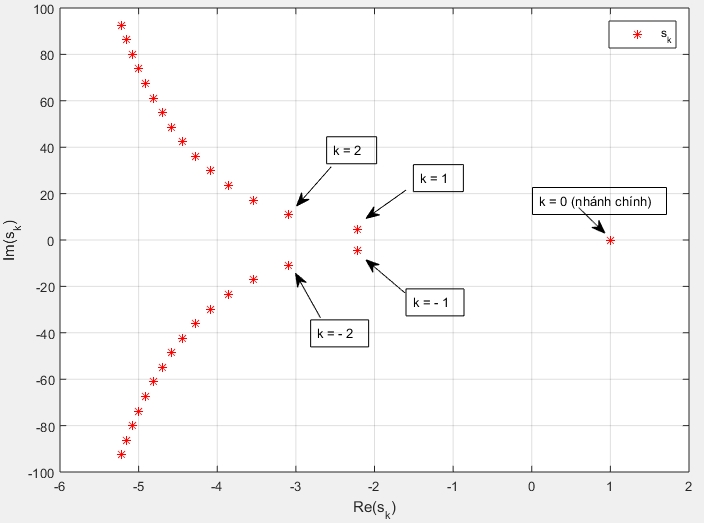
\includegraphics[width=0.8\linewidth]{hinh/hinh1}
	\caption{Giá trị riêng của phương trình \eqref{3} khi $a=-1, a_d=0.5,$ và $h=1$. Giá trị riêng bên phải là tương ứng với nhánh chính $k=0$, các cặp tiếp theo lần lượt tương ứng với $k=\pm 1, \ \pm 2, \dots, \pm 15$.}
	\label{refhinh1}
\end{figure}
\end{frame}

\begin{frame}
\begin{block}{Ví dụ 2.2}\label{vidu2} 
Xét hệ:  $\dot{x}(t)=(-1)x(t)+0.5x(t-1)+b\sin(t)$\\
Trong đó $x_0=1$ và $g(t)=1$ với $h=1$

\begin{table}[ht]
	\centering	
	\begin{tabular}{llll}
		\hline 
		k & $s_k$ & $C^I_k$ & $C^N_k$ \\ 
		\hline 
		0 & $-0.3149$ & 1.0713 & 0.5934 \\ 
		
		$\pm1$ & $-2.2211\mp4.442i$ & $-1.9829 \mp 0.4711i$ & $-0.0112\mp0.2245i$ \\ 
		
		$\pm2$ & $- 3.0915\mp10.8044i$ & $-2.0109 \mp 0.1863i$ & $- 0.0093\mp0.0916i$ \\ 
		
		$\pm3$ & $- 3.5450 \mp17.1313i$ & $-2.0073 \mp 0.1168i$ & $- 0.0052 \mp 0.0579i$ \\ 
		
		$\pm4$ & $-3.8550 \mp 23.4407i$ & $-2.0050 \mp 0.0852i$ & $-0.0034 \mp 0.0424i$  \\
		
		$\pm5$ & $ -4.0911 \mp 29.7416i$ & $-2.0036 \mp 0.0671i$ & $-0.0024 \mp 0.0335i$ \\
		
		\hline 
	\end{tabular}
	\caption{Các giá trị riêng và hệ số trong Ví dụ 2.2}
	\label{bang1} 
\end{table}%
\end{block}
\end{frame}

\begin{frame}
	\begin{figure}[ht]
	\begin{center}
		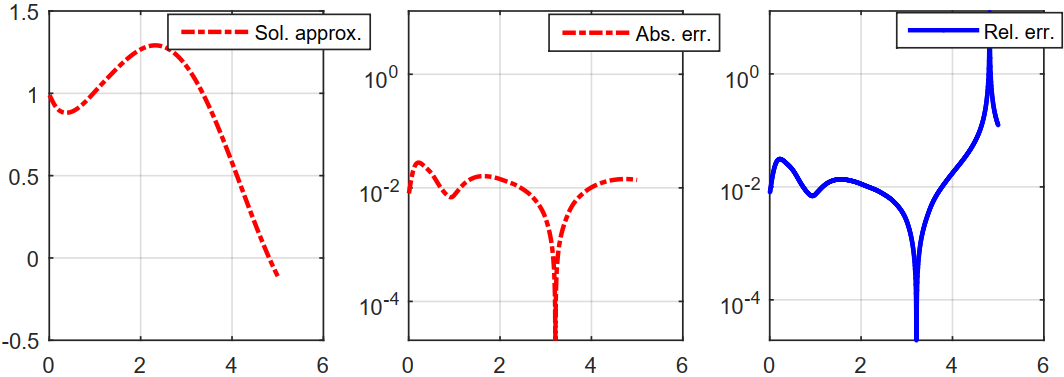
\includegraphics[scale=0.4]{hinh/hinh2}
	\end{center}
	\caption{Phản hồi cho trường hợp $u(t)=\sin(t)$, với $x_0=1$ và $g(t)=1$ cho $-h\leq t<0$, và so sánh giữa công thức chặt cụt nghiệm giữ 7 thành phần đầu tiên dựa trên phương pháp hàm Lambert (xem Bảng) và phương pháp số (hàm dde23 trong MATLAB). Các hệ số là $a=-1, a_d=0.5$, và $h=1$.}
	\label{refhinh2}
\end{figure}

Công thức nghiệm xấp xỉ
\begin{align*}
x(t) = \sum\limits^3_{k=-3}e^{S_kt}C^I_k+\int^t_0\sum\limits^3_{k=-3}e^{S_k(t-\eta)}C^N_kBu(\eta)d\eta
\end{align*}
%
\end{frame}


\subsection{Trường hợp hệ phương trình}

\begin{frame}{Trường hợp hệ phương trình}
Cho hệ điều khiển có trễ có dạng sau:
\begin{align*}\label{13}
\begin{split}
\dot{x}(t)&=Ax(t)+A_dx(t-h)+Bu(t), \\
y(t)&=Cx(t)+Du(t),
\end{split}
\end{align*}\pause
trong đó $x(t)$ là vectơ trạng thái, $u(t)$ là biến điều khiển, $y(t)$ là vectơ đầu ra,\ \pause $A, A_d, B, C$ và $D$ là các ma trận hệ số và $h$ là độ trễ vô hướng đã biết.\ \pause Điều kiện ban đầu $x(t=0)=x_0$ và $x(t)=g(t)$ với $-h\leq t <0$ phải được cho trước. \\ \pause
Công thức nghiệm cho hệ có dạng:
%
\begin{equation*}\label{14}
x(t) = \sum\limits^\infty_{k=-\infty}e^{S_kt}C^I_k+\int^t_0\sum\limits^\infty_{k=-\infty}e^{S_k(t-\eta)}C^N_kBu(\eta)d\eta,
\end{equation*} \pause
trong đó
\begin{equation*}\label{15}
S_k=\dfrac{1}{h}W_k(A_dhQ_k)+A,
\end{equation*} \pause
và $Q_k$ được lấy từ nghiệm số (như bằng cách sử dụng hàm $fsolve$ trong MATLAB) của phương trình
%
\begin{equation*}\label{16}
W_k(A_dhQ_k)e^{W_k(A_dhQ_k)+Ah}=A_dh.
\end{equation*} 
\end{frame}


\begin{frame}{}
\begin{block}{Ví dụ 2.3} 
	Cho
	\begin{equation*}
	\dot{x}(t) =
	\begin{bmatrix}
	-1&-3 \\
	2&-5
	\end{bmatrix}x(t)+ \  
	\begin{bmatrix}
	1.66&-0.697\\
	0.93&-0.33
	\end{bmatrix}x(t-1)
	+Bu(t)
	% Bu = \m{\cos(t) \\ \sin(t) }, \ 
	\end{equation*}\pause
	Để tìm các ma trận $S_k$ chúng ta sẽ sử dụng hàm $find\_Sk$ trong gói công cụ LambertWDDE.\ \pause
	Đối với nhánh chính, $k = 0$, ta có được :
	\begin{align*}
	S_0=\begin{bmatrix}
	0.3055&-1.4150\\
	2.1317&-3.3015
	\end{bmatrix} \ ,  \ 
	C^I_0=\begin{bmatrix}
	0.2635\\
	0.4290
	\end{bmatrix}.
	\end{align*}\pause
%
Do đó, phép xấp xỉ sử dụng một nhánh $k = 0$ cho phản hồi tự do là:
\begin{align*}
x(t)=\begin{bmatrix}
x_1(t)\\
x_2(t)
\end{bmatrix}
= exp \left(
\begin{bmatrix}
0.3055&-1.4150\\
2.1317&-3.3015
\end{bmatrix} t
\right)
\ 
\begin{bmatrix}
0.2635\\
0.4290
\end{bmatrix}.
\end{align*}
%
\end{block}
\end{frame}



\begin{frame}{}
Các nhánh $k=\pm 1$ cho ta các ma trận $S_k$ liên hợp phức bổ sung:
	\begin{align*}
	S_{-1,+1}=\begin{bmatrix}
	-0.3499\pm 4.980i&-1.6253\pm 0.1459i\\
	2.4174\pm 0.1308i&-5.1048\pm 4.5592i
	\end{bmatrix},
	\end{align*}
	với các hệ số liên hợp phức cho phản hồi tự do với $k = \pm 1$ là:
	\begin{align*}
	C^I_{-1,+1}=\begin{bmatrix}
	0.0909\pm 0.1457i\\
	0.0435\pm 0.1938i
	\end{bmatrix}.
	\end{align*}
	Công thức nghiệm xấp xỉ
	\begin{align*}
		x(t) = \sum\limits^1_{k=-1}e^{S_kt}C^I_k+\int^t_0\sum\limits^1_{k=-1}e^{S_k(t-\eta)}C^N_kBu(\eta)d\eta
	\end{align*}
%
\end{frame}

\begin{frame}
	\begin{center}
		\begin{figure}
			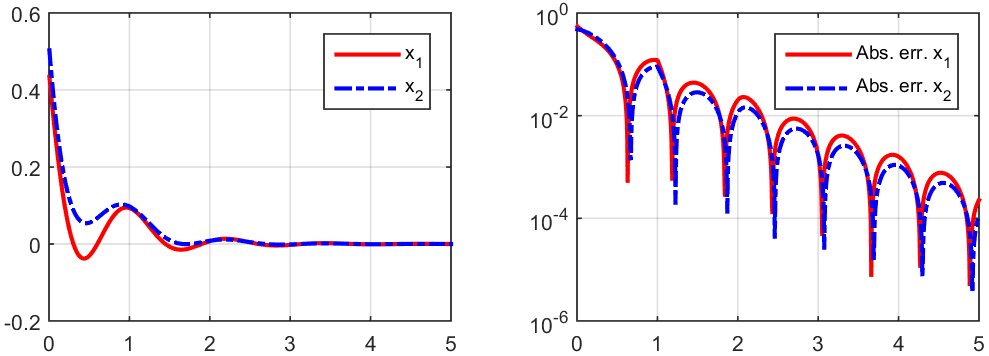
\includegraphics[scale=0.4]{hinh/hinh3_new.png}
			\caption{Phản hồi gần đúng (3 thành phần) và sai số tuyệt đối cho hệ trong Ví dụ 2.3
				so với nghiệm sử dụng hàm dựng sẵn dde23 trong MATLAB}
			\label{refhinh3}
		\end{figure}
	\end{center}
\end{frame}


%%%%%%%%%%%%%%%%%%%%%%%%%%%%%%%%%%%
\section{Tính ổn định của hệ}
\begin{frame}{Tính ổn định của hệ}
	\begin{block}{}
		Đối với các hệ thống có trễ tập phổ
	%
	\begin{equation*}\label{spectrum}
	\sigma(I,A,A_d) := \{\lb \in \mathbb{C} \ | \ \det(\lb I - A - e^{-\lb h}A_d ) = 0\}
	\end{equation*}
	%
	là vô hạn. Ta biết rằng với mọi số thực $\a$ luôn chỉ có một số hữu hạn các giá trị riêng nằm ở nửa mặt phẳng phải 
	$\C^+_{\a}:= \{ \a \in \C \ | \ \Re{\lb}\geq \a \}$.
	Chú ý rằng với $\a=0$ thì các giá trị riêng nằm trong $\C^+_{0}$ xác định sự ổn định của hệ thống.
		
	\end{block}\pause
	
	\begin{block}{Phỏng đoán 2.4}
		Xét hệ \begin{align*}
		\begin{split}
		\dot{x}(t)&=Ax(t)+A_dx(t-h)+Bu(t), \\
		y(t)&=Cx(t)+Du(t),
		\end{split}
		\end{align*}
		a) Giả sử rằng $0$ không phải là giá trị riêng bội của 
		ma trận hệ số $A_d$. Khi đó các giá trị riêng nằm trên nhánh chính $k=0$ sẽ có phần thực lớn nhất. \\
		b) Nếu $0$ là giá trị riêng bội của ma trận hệ số $A_d$ thì các giá trị riêng nằm trên ba nhánh bao gồm nhánh chính $k=0$ và hai nhánh $k=\pm 1$ sẽ có phần thực lớn nhất.
	\end{block}
\end{frame}

%%%%%%%%%%%%%%%%%%%%%%%%%%%%%%%%%%%
\section{Hàm phân rã cho hệ điều khiển có trễ}

\begin{frame}{Hàm phân rã cho hệ điều khiển có trễ}
	Mục tiêu là tìm ra giới hạn trên chặt cho tốc độ phân rã, được gọi là $\alpha$ - ổn định, cũng như giới hạn trên của hệ số $K$, sao cho chuẩn của biến trạng thái bị chặn 
	\begin{equation}\label{17}
	\Vert x(t)\Vert\leq Ke^{\alpha t}\Phi(h,t_0),
	\end{equation} 
	trong đó $\Phi(h,t_0)=\sup\limits_{t_0-h\leq t\leq t_0}\{\Vert x(t)\Vert\}$ và $\Vert \cdot\Vert$ biểu thị chuẩn Euclid. \\
	Sử dụng công thức nghiệm \eqref{14} ta có thể thu được ước lượng tối ưu của $\alpha$.	
\end{frame}



%%%%%%%%%%%%%%%%%%%%%%%%%%%%%%%%%%
\section{Tính điều khiển được và tính quan sát được}

\begin{frame}{Tính điều khiển được và tính quan sát được}
Xét hệ phương trình vi phân với trễ hằng số $h>0$ có dạng
%
\begin{align}\label{t1}
\dot{x}(t) &=  A x(t)  + A_d x(t-h)+B u(t) \mbox{ với mọi  } t>0 \notag \\
x(t) &= \begin{cases}
& g(t) \mbox{ với mọi  } t\in[-h,0) \\
& x_0         \mbox{ nếu } t = 0
\end{cases} \\
y(t)&=  C x(t),  \notag 
\end{align}
%
\end{frame}

\subsection{Tính điều khiển được}

\begin{frame}{Tính điều khiển được}
\begin{block}{Định nghĩa 4} 
	 Hệ \begin{align*}
	 \begin{split}
	 \dot{x}(t)&=Ax(t)+A_dx(t-h)+Bu(t), \\
	 y(t)&=Cx(t)+Du(t),
	 \end{split}
	 \end{align*} được gọi là {\it điều khiển được theo điểm} nếu với mọi điều kiện ban đầu $g(t)$ và $x_0$, tồn tại một thời điểm $t_1,0<t_1<\infty$ và một hàm chấp nhận được  $u(t)$, sao cho $x(t_1;g,x_0,u(t))=0$. 
\end{block}
\begin{block}{Định nghĩa 5} Hệ \eqref{t1} được gọi là \textit{đầy đủ theo điểm} (pointwise complete) tại thời điểm $t_1$ nếu với mọi $x_1\in \mathbb{R}^n$, tồn tại điều kiện ban đầu $g(t)$ và $x_0$ sao cho $x(t_1;g,x_0,0)=x_1$, với $x(t_1;g,x_0,0)$ là nghiệm của \eqref{t1} bắt đầu tại thời điểm $t=0$.
\end{block}	
\end{frame}


\begin{frame}{}
	\begin{block}{Định lý 2.6 (M. Malek-Zavarei và M. Jamshidi. 87)}
		Xét hệ điều khiển có trễ dạng \eqref{t1}. Khi đó hệ là đầy đủ theo điểm nếu như một trong các điều kiện đủ sau đây được thỏa mãn.
		\begin{enumerate}
			\item[i)] Cỡ của hệ là $2\times 2$. 
			\item[ii)] Hệ có ma trận hệ số $A_d$ không suy biến.
			\item[iii)] Hai ma trận $A$ và $A_d$ là giao hoán.
			\item[iv)] Tồn tại hai vector $a$ và $b$ thuộc $\R^{n,1}$ sao cho 
			$A_d = a b^T$.
		\end{enumerate}
	\end{block}
	
	\begin{block}{Chú ý 2.7}
		Trường hợp hệ không trễ ($A_d=0$) thì điều kiện iii) hiển nhiên thỏa mãn. Do đó tính điều khiển được hay quan sát được của hệ quay trở lại các tính chất tương ứng đã biết của hệ điều khiển tuyến tính không trễ.
	\end{block}
\end{frame}	


\begin{frame}{}
	\begin{block}{Định lý 2.8}
		Nếu hệ \eqref{t1} là đầy đủ theo điểm thì nó là điều khiển được theo điểm tới thời điểm $t_1 > 0$ khi và chỉ khi\pause
		\begin{equation}\label{t8}
		\text{rank}\left[\mathcal{C}(0,t_1)\equiv \int^{t_1}_0\sum\limits^\infty_{k=-\infty}e^{\mathbf{S}_k(t_1-\xi)}C^N_k {BB}^T\left(\sum\limits^\infty_{k=-\infty}e^{\mathbf{S}_k(t_1-\xi)}C^N_k\right)^Td\xi\right]=n,
		\end{equation}\pause
		với \ $\mathcal{C}(0,t_1)$ \ là \textit{ma trận điều khiển Gramian} của hệ và chỉ số trên \ $^T$ chỉ hoán vị của một ma trận.
	\end{block}		
\end{frame}	


\begin{frame}{}
		\begin{block}{Định nghĩa 6}
			Một tập hợp hữu hạn các hàm giá trị vector $f_1(t),\dots,f_n(t)$ trên cùng một miền xác định $\mathbb{D} \subseteq \R$ được gọi là phụ thuộc tuyến tính trên trường $\mathbb{K}$ nếu tồn tại các số $c_1,\dots,c_n \in \mathbb{K}$ và không đồng thời bằng $0$ sao cho
			%
			\[
			c_1 f_1(t) + c_2 f_2(t) + \dots + c_n f_n(t) = 0 \ \mbox{ với mọi } \ t\in \mathbb{D} \ .
			\]
			%
			Ngược lại thì tập các hàm nói trên được gọi là độc lập tuyến tính.
		\end{block}
	
	\begin{block}{Bổ đề 2.10 (Chen'98)}
		Cho hàm giá trị ma trận $F(t)$ xác định trên đoạn $[t_1,t_2] \subset \R$. Khi đó các hàng của $F(t)$ là độc lập tuyến tính trên đoạn $[t_1,t_2]$ khi và chỉ khi ma trận $\cP(t_1,t_2) := \int_{t_1}^{t_2} F(t)F^T(t)$ là khả nghịch.
		\end{block}
\end{frame}

%
\begin{frame}{}	
		\begin{block}{Hệ quả 2.11}
			Hệ \eqref{t1} là điều khiển được theo điểm khi và chỉ khi tất cả các cột của ma trận
			\begin{equation}\label{t13}
			\sum\limits^\infty_{k=-\infty}e^{\mathbf{S}_k(t-0)}C^N_kB,
			\end{equation}
			là độc lập tuyến tính trên $[0,\infty)$.
		\end{block}
		\begin{block}{Hệ quả 2.12}        
			Hệ \eqref{t1} là tính điều khiển được theo điểm khi và chỉ khi tất cả các hàng của ma trận
			\begin{equation}\label{t15}
			(s\mathbf{I}-A-A_de^{-sh})^{-1}B 
			\end{equation} 	  
			là độc lập tuyến tính trên tập tất cả mọi số phức $s$ không thuộc phổ của hệ \eqref{t1}.
		\end{block}	 
\end{frame}

\subsection{Tính quan sát được}

\begin{frame}{Tính quan sát được}
	\begin{block}{Định nghĩa 7}
		Hệ 
		\begin{align*}
		\begin{split}
		\dot{x}(t)&=Ax(t)+A_dx(t-h)+Bu(t), \\
		y(t)&=Cx(t)+Du(t),
		\end{split}
		\end{align*}
	được gọi là {\it quan sát được theo điểm} trong $[0, t_1]$ nếu điều kiện ban đầu $x_0$ có thể được xác định duy nhất từ $u(t)$, $g(t)$, và $y(t)$.
	\end{block}
	\begin{block}{Định lý 2.14}
		Hệ \eqref{t1} là quan sát được theo điểm khi và chỉ khi
		%	  
		\begin{equation}\label{t16}
		rank\left[\mathcal{O}(0,t_1)\equiv rank\int^{t_1}_0\left(\sum\limits^\infty_{k=-\infty}e^{\mathbf{S}_k(\xi -0)}C^N_k\right)^TC^TC\sum\limits^\infty_{k=-\infty}e^{\mathbf{S}_k(\xi -0)}C^N_kd\xi \right]=n,
		\end{equation}\pause
		%
		trong đó $\mathcal{O}(0,t_1)$ là ma trận quan sát Gramian của hệ \eqref{t1}.
	\end{block}
\end{frame}


\begin{frame}{}
	\begin{block}{Hệ quả 2.15}
		Hệ \eqref{t1} là quan sát được theo điểm khi và chỉ khi tất cả các cột của ma trận
		\begin{equation}\label{t17}
		C\sum\limits^\infty_{k=-\infty}e^{\mathbf{S}_k(t-0)}C^N_k,
		\end{equation}	
		là độc lập tuyến tính.
	\end{block}
	
	\begin{block}{Hệ quả 2.16}
		Hệ \eqref{t1} là quan sát được theo điểm khi và chỉ khi tất cả các cột của ma trận
		\begin{equation}\label{t18}
		C(s\mathbf{I}-A-A_de^{-sh})^{-1}
		\end{equation}
		là độc lập tuyến tính ngoại trừ tại các điểm $s$ thuộc phổ của hệ \eqref{t1}.
	\end{block}
\end{frame}
%
\begin{frame}{}
\begin{block}{Ví dụ 2.18}
	Xét hệ \eqref{t1} với các tham số sau
		
	\begin{equation}\label{t19}
	A=\begin{bmatrix}
	-1 & -3\\
	2 & -5
	\end{bmatrix},\quad
	A_d=\begin{bmatrix}
	1.66 & -0.697\\
	0.93 & -0.330
	\end{bmatrix},\quad h=1 \ .
	\end{equation}
	Hệ \eqref{t19} là điều khiển được theo điểm. Cho $B=[1\quad 0]^T$ chúng ta có thể tính toán ma trận điều khiển được Gramian $\mathcal{C}(0,t_1)$ trong \eqref{t8}. 
	Do đó để hệ \eqref{t19} là điều khiển được theo điểm thì $\mathcal{C}(0,t_1)$ phải khả nghịch, tức là 
	%
	\begin{equation}\label{t20}
	\det C(0,t_1) \not= 0.
	\end{equation} 
\end{block}   
\end{frame}



\begin{frame}
\begin{minipage}{6.5cm} 
	\begin{figure}[t]
		\centering
		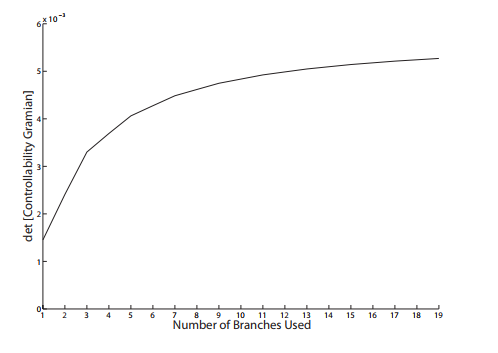
\includegraphics[width=0.7\linewidth]{hinh/hinh2n}
		\caption{Xấp xỉ định thức của ma trận điều khiển Gramian. Khi nhiều nhánh hơn được sử dụng, các định thức có xu hướng hội tụ về một giới hạn khác không.}
		\label{n.refhinh2}
	\end{figure} 
\end{minipage}
\hfill
\begin{minipage}{5cm}
	\begin{figure}[t]
		\centering
		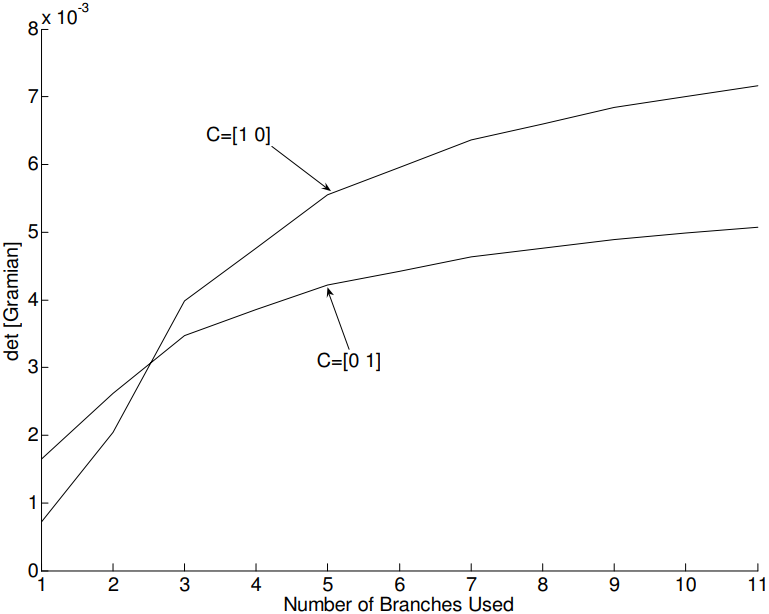
\includegraphics[width=0.6\linewidth]{hinh/hinh3n}
		\caption{Định thức của ma trận quan sát Gramian khi $C=[0\quad 1]$ và $C=[1\quad 0]$.}
		\label{n.refhinh3}
	\end{figure}   
\end{minipage}

\end{frame}


%%%%%%%%%%%%%%%%%%%%%%%%%%%%
\section{Phân tích và điều khiển các hệ có trễ sử dụng gói công cụ LambertWDDE}
\subsection{Phân tích sự rung lắc của máy công cụ}

\begin{frame}{Phân tích sự rung lắc của máy công cụ}
`	\begin{figure}[h!]
		\centering
		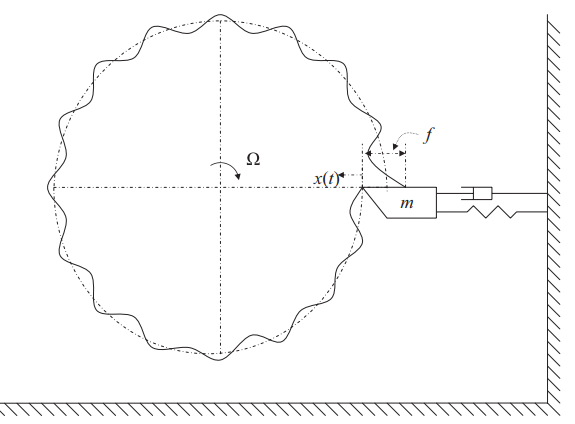
\includegraphics[width=0.7\linewidth]{hinh/machine_tool_chatter}
		\caption{Mô hình máy cắt vuông góc một bậc tự do}
		\label{fig:machinetoolchatter}
	\end{figure}
\end{frame}


\begin{frame}
	Hệ
	\begin{align*}\label{turning proceess 2}
	\dot{x}_1(t) &= x_2(t), \notag \\
	\dot{x}_2(t) &= 2 \xi \omega_n {x}_2(t) + \left( \omega_n^2 + \dfrac{k_c}{m}\right) x_1(t) - \dfrac{k_c}{m} x_1(t-\tau ) \notag \\
	& \quad + \dfrac{k_c}{8 f_0 m} \left( (x_1(t) - x_1(t-\tau) )^2 - \dfrac{5}{12 f_0} (x_1(t) - x_1(t-\tau) )^3 \right),  
	\end{align*}
	%
	Giả sử rằng không có dao động nào trong vòng tiện trước, tức là $x_1(t-\tau) = 0$, thì điểm cân bằng là $x_1(t)=x_2(t) = 0$, 
	có nghĩa là cạnh dao nằm tại vị trí như được xác định trước đó.\\
	Tuyến tính hóa hệ tại điểm cân bằng 
	
	với $k_m := m \omega_n^2$ là \emph{độ cứng cấu trúc} (N/m), ta có hệ
	%
	\begin{equation}\label{eq4}
	\m{\dot{x}_1(t) \\ \dot{x}_2(t)} = \m{0 & 1 \\ - \omega_n^2 \left( 1 + \dfrac{k_c}{k_m}\right) & - 2 \xi \omega_n } \m{{x}_1(t) \\ {x}_2(t)} 
	+ \m{0 & 0 \\ \dfrac{k_c}{k_m}\omega_n^2 & 0 } \m{{x}_1(t-\tau) \\ {x}_2(t-\tau)} \ .
	\end{equation}
	%
	Sự rung lắc sẽ xảy ra nếu như hệ \eqref{eq4} không ổn định.
\end{frame}

\begin{frame}
	Ví dụ ta xét trường hợp tốc độ quay trục chính $1/T$ = 50, $\omega_n = 150$ ($Hz^2$) và $\xi = 0.05$, tỉ số $\dfrac{k_c}{k_m} = 0.25$.
	Khi đó các ma trận $S_k$ và các giá trị riêng tương ứng thu được qua tính toán là như trong Bảng \ref{bang 3}.
	
	\begin{table}[!h]
		\centering
		\begin{tabular}{lcc}
			\hline \\[-.35cm]	
			Chỉ số nhánh & $S_{k_1,k_2}$ & Giá trị riêng của $S_{k_1,k_2}$ \\ \hline \\[-.35cm]
			$k_1 = k_2 = 0$		   & $\m{0 & 1 \\ -33083 & -0.24}$ & $-0.12 \pm 181.88 i$ \\ \hline \\[-.35cm]
			$k_1 = -1$, $k_2 = 0$  & $\m{0 & 1 \\ -77988 + 32093i & -177 - 247i }$ &  
			$\pma{- 0.12 + 181.88 i \\ -176.73 - 428.66i}$ \\ 
			$k_1 = 0$, $k_2 = -1$	& $\m{0 & 1 \\ -11 - 1663i & -92 - 182i}$  &  $\pma{ -91.61 \\ - 0.12-181.88i}$ \\ \hline \\[-.35cm]
			$k_1 = 1$, $k_2 = 0$   & $\m{0 & 1 \\ -77988 - 32093i & -177 + 247i}$ &  
			$\pma{- 0.12 - 181.88 i \\ -176.73 + 428.66i}$ \\ 
			$k_1 = 0$, $k_2 = 1$	& $\m{0 & 1 \\ -11 + 1663i & -92 + 182i}$  &  $\pma{ -91.61 \\ - 0.12-181.88i}$ \\ \hline \\[-.35cm]
			$\vdots$ & $\vdots$ & $\vdots$ \\ \hline
		\end{tabular} 
		\caption{Tính toán các ma trận $S_k$ và các giá trị riêng trội}
		\label{bang 3}
	\end{table}
Theo phỏng đoán 2.4 ta dự đoán rằng hệ là ổn định không điều kiện.
\end{frame}



\begin{frame}
	\begin{figure}[h!]
		\centering
		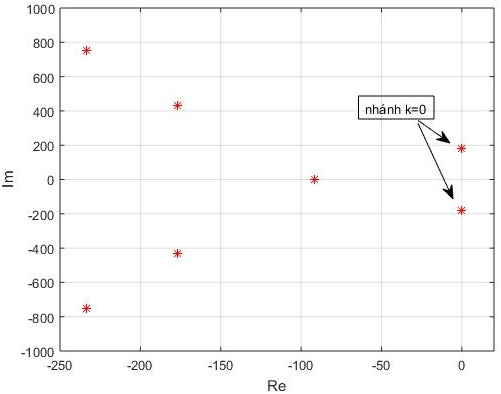
\includegraphics[width=0.7\linewidth]{hinh/spectrum_chatter-2}
		\caption{Giá trị riêng của hệ \eqref{eq4} trong mặt phẳng phức. Các giá trị riêng thu được bằng cách sử dụng nhánh chính (k = 0) là trội và sẽ quyết định tính ổn định của hệ.}
		\label{spectrumchatter-2}
	\end{figure}
\end{frame}

\begin{frame}
	\begin{figure}[h!]
		\centering
		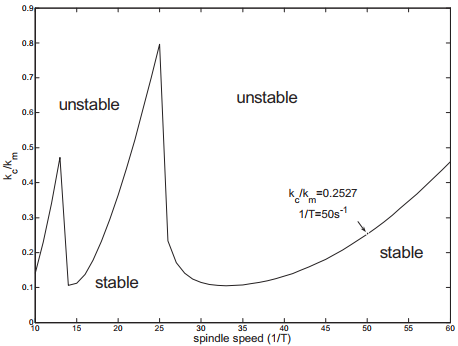
\includegraphics[width=0.8\linewidth]{hinh/stability-lobes}
		\caption{Các ngưỡng ổn định trong bài toán rung lắc của máy tiện}
		\label{fig:stability-lobes}
	\end{figure}
\end{frame}


%%%%%%%%%%%%%%%%%%%%%%%%%%%%%%%
\subsection{Điều khiển động cơ Diesel}

\begin{frame}{Điều khiển động cơ Diesel}
	\begin{figure}[h!]
		\centering
		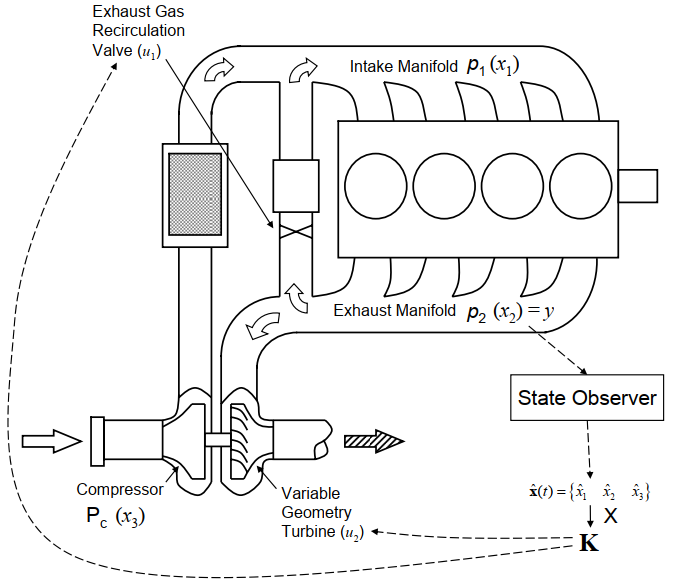
\includegraphics[scale=0.3]{hinh/diesel_engine_control}
		\caption{Điều khiển động cơ diesel bằng việc sử dụng đo đạc áp suất ống xả, tất cả các trạng thái đều sẽ được ước lượng thông qua bộ quan sát trạng thái và sau đó được sử dụng trong việc thiết kế điều khiển phản hồi }
		\label{fig:dieselenginecontrol}
	\end{figure}
\end{frame}


\begin{frame}
	Cho một điểm vận hành cụ thể (N = 1500 vòng/phút) có dạng
	%
	\begin{equation*}\label{eq7}
	\dot{x}(t) = \underbrace{\m{-27 & 3.6 & 6 \\ 9.6 & -12.5 & 0 \\ 0 & 9 & -5}}_{A} {x}(t) +   
	\underbrace{\m{0 & 0 & 0 \\ 21 & 0 & 0 \\0 & 0 & 0 }}_{A_d} {x}(t-h) + 
	\underbrace{\m{0.26 & 0 \\ -0.9 & -0.8 \\ 0 & 0.18}}_{B} {u}(t)  \ .
	\end{equation*}
	%
	 đầu ra là
	%
	\begin{equation*}\label{eq5}
	y(t) = \m{0 & 1 & 0} x(t) \ .
	\end{equation*}
	
\end{frame}

\begin{frame}
	\begin{figure}[h!]
		\centering
		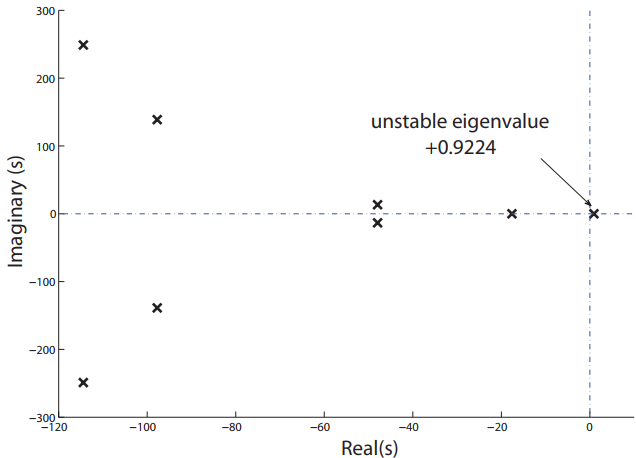
\includegraphics[width=0.7\linewidth]{hinh/spectrum_diesel}
		\caption{Phổ của hệ \eqref{eq7}.}
		\label{fig:spectrumdiesel}
	\end{figure}
\end{frame}


\begin{frame}
	 Ví dụ, để xét tính điều khiển được, ta có thể sử dụng gói công cụ Symbolic trong MATLAB để tính toán trực tiếp
	%
	\begin{equation*}
	(s\mathbf{I}-A-A_d e^{-sh})^{-1}B 
	= \m{ s + 27 &    -18/5 &    -6 \\ - 21 e^{-sh} - 48/5 & s + 25/2 &     0 \\ 0 & -9 & s + 5 }^{-1} \m{0.26 & 0 \\ -0.9 & -0.8 \\ 0 & 0.18}, 
	\end{equation*}
	%
	và kiểm tra điều kiện hạng \eqref{t15}. Đó là cách làm được thực hiện trong hàm \linebreak \emph{pwcontr\_test} trong gói công cụ LambertWDDE.
	Điều tương tự cũng được thực hiện với tính quan sát được, sử dụng 
	hàm \emph{pwobs\_test} trong cùng gói công cụ. \ 
	Khi đó, hệ điều khiển có trễ vừa là điều khiển được theo điểm vừa là quan sát được theo điểm. Điều này phù hợp với những quan sát trong thực tế.
\end{frame}

%%%%%%%%%%%%%%%%%%%%%
\begin{frame}{KẾT LUẬN}
	Luận văn đã trình bày phương pháp tiếp cận và sử dụng hàm Lambert để cho các hệ điều khiển có trễ để:
	\begin{itemize}
		 		 \item Tìm công thức nghiệm tường minh và nghiệm xấp xỉ
		 \item Áp dụng trong việc nghiên cứu tính ổn định và tính phân ra của hệ
		 \item Áp dụng để nghiên cứu tính điều khiển được và tính quan sát được của hệ
		 \item Áp dụng vào các ví dụ thực tế
	\end{itemize}\pause
Mục tiêu tương lai:\\
Áp dụng phương pháp hàm Lambert cho các hệ có trễ trung tính và các hệ vi phân đại số
\end{frame}




%%%%%%%%%%%%%%%%%%%%%%%%%%%%%%
\begin{frame}
\begin{center}
	
	\textbf{\Large EM XIN CHÂN THÀNH CẢM ƠN!}
	
\end{center}
\end{frame}



%%%%%%%%%%Phần này thêm cho chạy chỉ dẫn tài liệu tham khảo48
%\begin{frame}{Tài liệu tham khảo}

%\addcontentsline{toc}{chapter}{TÀI LIỆU THAM KHẢO}
\centerline{\bf TÀI LIỆU THAM KHẢO\markboth{\sc TÀI LIỆU THAM KHẢO}{}}
\begin{thebibliography}{99}
\bibitem{Chen98} C. T. Chen. \textit{Linear System Theory and Design}. Oxford University Press 1998,

\bibitem{Mal87} M. Malek-Zavarei and Mohammad Jamshidi. \textit{Time-Delay Systems: Analysis, Optimization and Applications}. NewYork, USA: Elservier Science Pub, 1987,

\bibitem{Yi12} S. Yi, S. Duan, P.W. Nelson, A.G. Ulsoy,
\textit{The Lambert W Function Approach to Time Delay Systems and the LambertW\_DDE Toolbox},
IFAC Proceedings Volumes,
Volume 45, Issue 14,
2012,

\bibitem{Yi07} S. Yi, P. W. Nelson, and A. G. Ulsoy. Delay differential equations via the
matrix Lambert W function and bifurcation analysis: application to machine
tool chatter.\textit{Mathematical Biosciences and Engineering}, 2007,

\bibitem{Yi08} S. Yi, P. W. Nelson, and A. G. Ulsoy. Controllability and observability of systems of linear delay differential equations via the matrix Lambert W function.
\textit{IEEE Trans. Automatic Control}, 2008,


\bibitem{Yi10} S. Yi, P. W. Nelson, and A. G. Ulsoy.  \textit{Time-Delay Systems: Analysis and
Control Using the Lambert W Function}. World Scientific, 2010,



\end{thebibliography}
%\end{frame}
%%%%%%%%%%%%%%%%%%%%%%%%%%%%%%%%%%%%%%%%%%%%%

\end{document}

%%14:20:25 8/1/2015Last Modification of contents
%%13:1:33 10/1/2015Last Modification of contents